% Created by tikzDevice version 0.12.3.1 on 2022-06-27 14:34:14
% !TEX encoding = UTF-8 Unicode
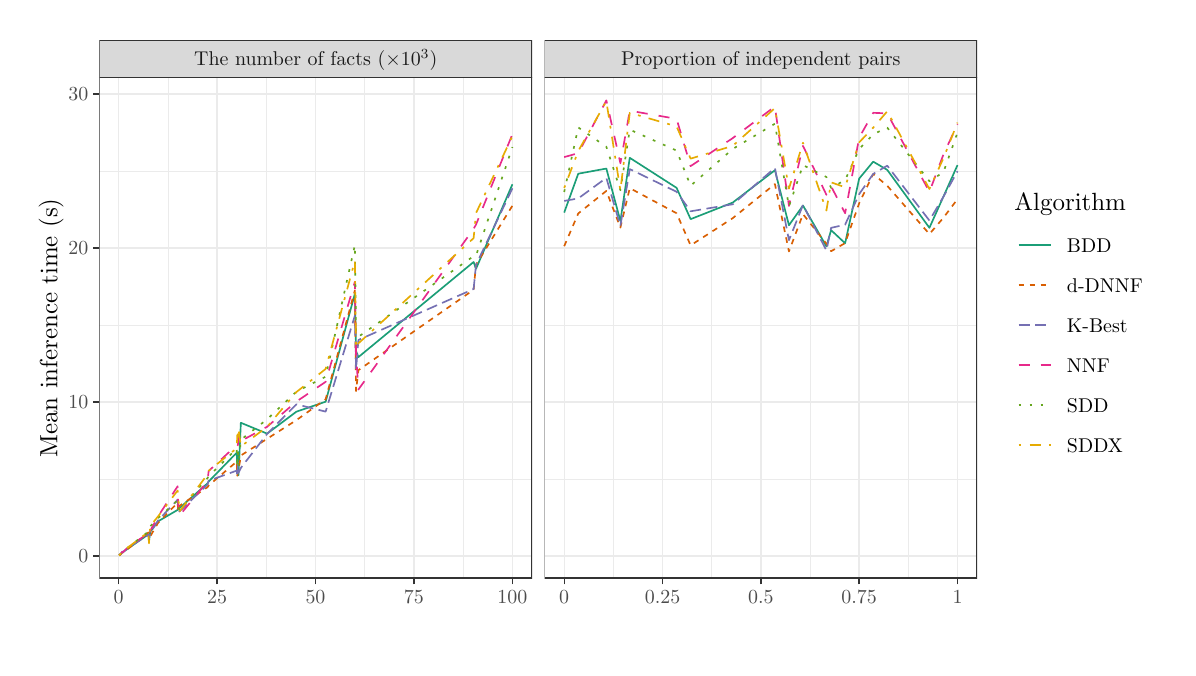
\begin{tikzpicture}[x=1pt,y=1pt]
\definecolor{fillColor}{RGB}{255,255,255}
\path[use as bounding box,fill=fillColor,fill opacity=0.00] (0,0) rectangle (411.94,224.04);
\begin{scope}
\path[clip] (  0.00,  0.00) rectangle (411.94,224.04);
\definecolor{drawColor}{RGB}{255,255,255}
\definecolor{fillColor}{RGB}{255,255,255}

\path[draw=drawColor,line width= 0.5pt,line join=round,line cap=round,fill=fillColor] (  0.00,  0.00) rectangle (411.94,224.04);
\end{scope}
\begin{scope}
\path[clip] ( 25.95, 25.11) rectangle (182.27,205.98);
\definecolor{fillColor}{RGB}{255,255,255}

\path[fill=fillColor] ( 25.95, 25.11) rectangle (182.27,205.98);
\definecolor{drawColor}{gray}{0.92}

\path[draw=drawColor,line width= 0.2pt,line join=round] ( 25.95, 61.00) --
	(182.27, 61.00);

\path[draw=drawColor,line width= 0.2pt,line join=round] ( 25.95,116.62) --
	(182.27,116.62);

\path[draw=drawColor,line width= 0.2pt,line join=round] ( 25.95,172.24) --
	(182.27,172.24);

\path[draw=drawColor,line width= 0.2pt,line join=round] ( 50.63, 25.11) --
	( 50.63,205.98);

\path[draw=drawColor,line width= 0.2pt,line join=round] ( 86.21, 25.11) --
	( 86.21,205.98);

\path[draw=drawColor,line width= 0.2pt,line join=round] (121.79, 25.11) --
	(121.79,205.98);

\path[draw=drawColor,line width= 0.2pt,line join=round] (157.37, 25.11) --
	(157.37,205.98);

\path[draw=drawColor,line width= 0.5pt,line join=round] ( 25.95, 33.19) --
	(182.27, 33.19);

\path[draw=drawColor,line width= 0.5pt,line join=round] ( 25.95, 88.81) --
	(182.27, 88.81);

\path[draw=drawColor,line width= 0.5pt,line join=round] ( 25.95,144.43) --
	(182.27,144.43);

\path[draw=drawColor,line width= 0.5pt,line join=round] ( 25.95,200.05) --
	(182.27,200.05);

\path[draw=drawColor,line width= 0.5pt,line join=round] ( 32.84, 25.11) --
	( 32.84,205.98);

\path[draw=drawColor,line width= 0.5pt,line join=round] ( 68.42, 25.11) --
	( 68.42,205.98);

\path[draw=drawColor,line width= 0.5pt,line join=round] (104.00, 25.11) --
	(104.00,205.98);

\path[draw=drawColor,line width= 0.5pt,line join=round] (139.58, 25.11) --
	(139.58,205.98);

\path[draw=drawColor,line width= 0.5pt,line join=round] (175.16, 25.11) --
	(175.16,205.98);
\definecolor{drawColor}{RGB}{27,158,119}

\path[draw=drawColor,line width= 0.6pt,line join=round] ( 33.05, 33.37) --
	( 33.27, 33.52) --
	( 33.69, 33.91) --
	( 34.26, 34.58) --
	( 34.55, 34.59) --
	( 36.25, 35.83) --
	( 43.62, 40.94) --
	( 43.83, 38.43) --
	( 44.26, 41.84) --
	( 47.07, 45.62) --
	( 54.19, 49.79) --
	( 54.40, 49.96) --
	( 54.83, 50.42) --
	( 64.97, 59.37) --
	( 65.40, 60.03) --
	( 75.54, 70.46) --
	( 75.75, 64.76) --
	( 75.96, 70.64) --
	( 76.18, 62.32) --
	( 77.03, 81.27) --
	( 86.53, 77.35) --
	( 97.10, 85.28) --
	(107.67, 88.88) --
	(118.23,127.89) --
	(118.66,107.19) --
	(119.51,105.00) --
	(161.14,139.37) --
	(162.00,136.90) --
	(175.16,167.44);
\definecolor{drawColor}{RGB}{217,95,2}

\path[draw=drawColor,line width= 0.6pt,dash pattern=on 2pt off 2pt ,line join=round] ( 33.05, 33.33) --
	( 33.27, 33.46) --
	( 33.69, 33.82) --
	( 34.26, 34.50) --
	( 34.55, 34.44) --
	( 36.25, 35.73) --
	( 43.62, 41.62) --
	( 43.83, 40.00) --
	( 44.26, 40.20) --
	( 47.07, 45.01) --
	( 54.19, 52.39) --
	( 54.40, 49.18) --
	( 54.83, 51.24) --
	( 64.97, 57.99) --
	( 65.40, 58.62) --
	( 75.54, 67.23) --
	( 75.75, 62.11) --
	( 75.96, 63.39) --
	( 76.18, 64.01) --
	( 77.03, 69.44) --
	( 86.53, 75.49) --
	( 97.10, 82.22) --
	(107.67, 89.78) --
	(118.23,129.12) --
	(118.66, 92.72) --
	(119.51,100.28) --
	(161.14,129.33) --
	(162.00,138.38) --
	(175.16,159.71);
\definecolor{drawColor}{RGB}{117,112,179}

\path[draw=drawColor,line width= 0.6pt,dash pattern=on 4pt off 2pt ,line join=round] ( 33.05, 33.38) --
	( 33.27, 33.64) --
	( 33.69, 34.01) --
	( 34.26, 34.65) --
	( 34.55, 34.66) --
	( 36.25, 36.07) --
	( 43.62, 40.82) --
	( 43.83, 39.50) --
	( 44.26, 41.47) --
	( 47.07, 45.90) --
	( 54.19, 53.47) --
	( 54.40, 51.03) --
	( 54.83, 49.18) --
	( 64.97, 58.96) --
	( 65.40, 60.32) --
	( 75.54, 63.98) --
	( 75.75, 62.13) --
	( 75.96, 66.98) --
	( 76.18, 63.17) --
	( 77.03, 64.95) --
	( 86.53, 77.27) --
	( 97.10, 87.94) --
	(107.67, 85.30) --
	(118.23,119.94) --
	(118.66,100.54) --
	(119.51,111.19) --
	(161.14,129.60) --
	(162.00,138.33) --
	(175.16,165.99);
\definecolor{drawColor}{RGB}{231,41,138}

\path[draw=drawColor,line width= 0.6pt,dash pattern=on 4pt off 4pt ,line join=round] ( 33.05, 33.37) --
	( 33.27, 33.53) --
	( 33.69, 33.97) --
	( 34.26, 34.71) --
	( 34.55, 34.58) --
	( 36.25, 36.25) --
	( 43.62, 41.37) --
	( 43.83, 40.30) --
	( 44.26, 42.18) --
	( 47.07, 47.37) --
	( 54.19, 58.32) --
	( 54.40, 51.70) --
	( 54.83, 47.71) --
	( 64.97, 60.10) --
	( 65.40, 63.85) --
	( 75.54, 73.21) --
	( 75.75, 73.00) --
	( 75.96, 73.21) --
	( 76.18, 76.81) --
	( 77.03, 74.66) --
	( 86.53, 79.83) --
	( 97.10, 88.93) --
	(107.67, 96.07) --
	(118.23,132.20) --
	(118.66,105.84) --
	(119.51, 93.28) --
	(161.14,151.35) --
	(162.00,152.87) --
	(175.16,185.57);
\definecolor{drawColor}{RGB}{102,166,30}

\path[draw=drawColor,line width= 0.6pt,dash pattern=on 1pt off 3pt ,line join=round] ( 33.05, 33.41) --
	( 33.27, 33.58) --
	( 33.69, 33.98) --
	( 34.26, 34.75) --
	( 34.55, 34.67) --
	( 36.25, 36.24) --
	( 43.62, 41.94) --
	( 43.83, 43.49) --
	( 44.26, 43.83) --
	( 47.07, 46.77) --
	( 54.19, 53.21) --
	( 54.40, 51.40) --
	( 54.83, 49.70) --
	( 64.97, 61.26) --
	( 65.40, 61.93) --
	( 75.54, 71.92) --
	( 75.75, 65.30) --
	( 75.96, 70.93) --
	( 76.18, 65.57) --
	( 77.03, 75.13) --
	( 86.53, 82.53) --
	( 97.10, 92.52) --
	(107.67, 97.91) --
	(118.23,145.49) --
	(118.66,114.18) --
	(119.51,112.35) --
	(161.14,141.46) --
	(162.00,141.66) --
	(175.16,180.91);
\definecolor{drawColor}{RGB}{230,171,2}

\path[draw=drawColor,line width= 0.6pt,dash pattern=on 1pt off 3pt on 4pt off 3pt ,line join=round] ( 33.05, 33.33) --
	( 33.27, 33.61) --
	( 33.69, 33.96) --
	( 34.26, 34.72) --
	( 34.55, 34.69) --
	( 36.25, 36.23) --
	( 43.62, 41.81) --
	( 43.83, 37.71) --
	( 44.26, 43.93) --
	( 47.07, 47.37) --
	( 54.19, 56.79) --
	( 54.40, 54.58) --
	( 54.83, 49.17) --
	( 64.97, 62.57) --
	( 65.40, 63.92) --
	( 75.54, 72.06) --
	( 75.75, 76.85) --
	( 75.96, 74.63) --
	( 76.18, 79.27) --
	( 77.03, 72.70) --
	( 86.53, 79.83) --
	( 97.10, 92.37) --
	(107.67,100.72) --
	(118.23,139.80) --
	(118.66,108.14) --
	(119.51,109.97) --
	(161.14,147.98) --
	(162.00,157.02) --
	(175.16,184.87);
\definecolor{drawColor}{gray}{0.20}

\path[draw=drawColor,line width= 0.5pt,line join=round,line cap=round] ( 25.95, 25.11) rectangle (182.27,205.98);
\end{scope}
\begin{scope}
\path[clip] (186.77, 25.11) rectangle (343.09,205.98);
\definecolor{fillColor}{RGB}{255,255,255}

\path[fill=fillColor] (186.77, 25.11) rectangle (343.09,205.98);
\definecolor{drawColor}{gray}{0.92}

\path[draw=drawColor,line width= 0.2pt,line join=round] (186.77, 61.00) --
	(343.09, 61.00);

\path[draw=drawColor,line width= 0.2pt,line join=round] (186.77,116.62) --
	(343.09,116.62);

\path[draw=drawColor,line width= 0.2pt,line join=round] (186.77,172.24) --
	(343.09,172.24);

\path[draw=drawColor,line width= 0.2pt,line join=round] (211.64, 25.11) --
	(211.64,205.98);

\path[draw=drawColor,line width= 0.2pt,line join=round] (247.17, 25.11) --
	(247.17,205.98);

\path[draw=drawColor,line width= 0.2pt,line join=round] (282.69, 25.11) --
	(282.69,205.98);

\path[draw=drawColor,line width= 0.2pt,line join=round] (318.22, 25.11) --
	(318.22,205.98);

\path[draw=drawColor,line width= 0.5pt,line join=round] (186.77, 33.19) --
	(343.09, 33.19);

\path[draw=drawColor,line width= 0.5pt,line join=round] (186.77, 88.81) --
	(343.09, 88.81);

\path[draw=drawColor,line width= 0.5pt,line join=round] (186.77,144.43) --
	(343.09,144.43);

\path[draw=drawColor,line width= 0.5pt,line join=round] (186.77,200.05) --
	(343.09,200.05);

\path[draw=drawColor,line width= 0.5pt,line join=round] (193.87, 25.11) --
	(193.87,205.98);

\path[draw=drawColor,line width= 0.5pt,line join=round] (229.40, 25.11) --
	(229.40,205.98);

\path[draw=drawColor,line width= 0.5pt,line join=round] (264.93, 25.11) --
	(264.93,205.98);

\path[draw=drawColor,line width= 0.5pt,line join=round] (300.46, 25.11) --
	(300.46,205.98);

\path[draw=drawColor,line width= 0.5pt,line join=round] (335.99, 25.11) --
	(335.99,205.98);
\definecolor{drawColor}{RGB}{27,158,119}

\path[draw=drawColor,line width= 0.6pt,line join=round] (193.87,157.23) --
	(198.95,171.27) --
	(209.10,173.13) --
	(214.18,154.17) --
	(217.56,177.01) --
	(234.48,166.16) --
	(239.55,154.85) --
	(254.78,160.85) --
	(270.01,172.52) --
	(275.08,152.64) --
	(280.16,159.77) --
	(288.62,145.00) --
	(290.31,150.87) --
	(295.38,146.14) --
	(300.46,169.51) --
	(305.53,175.62) --
	(310.61,172.64) --
	(325.84,151.72) --
	(330.91,163.01) --
	(335.99,174.38);
\definecolor{drawColor}{RGB}{217,95,2}

\path[draw=drawColor,line width= 0.6pt,dash pattern=on 2pt off 2pt ,line join=round] (193.87,145.07) --
	(198.95,156.90) --
	(209.10,165.05) --
	(214.18,151.81) --
	(217.56,166.07) --
	(234.48,156.98) --
	(239.55,145.37) --
	(254.78,155.22) --
	(270.01,167.53) --
	(275.08,143.18) --
	(280.16,156.65) --
	(288.62,145.98) --
	(290.31,143.25) --
	(295.38,146.20) --
	(300.46,160.59) --
	(305.53,171.18) --
	(310.61,166.90) --
	(325.84,149.46) --
	(330.91,155.36) --
	(335.99,162.09);
\definecolor{drawColor}{RGB}{117,112,179}

\path[draw=drawColor,line width= 0.6pt,dash pattern=on 4pt off 2pt ,line join=round] (193.87,161.43) --
	(198.95,162.33) --
	(209.10,169.77) --
	(214.18,152.37) --
	(217.56,172.94) --
	(234.48,164.74) --
	(239.55,157.69) --
	(254.78,160.22) --
	(270.01,173.36) --
	(275.08,147.24) --
	(280.16,159.97) --
	(288.62,143.54) --
	(290.31,151.70) --
	(295.38,152.85) --
	(300.46,163.90) --
	(305.53,171.18) --
	(310.61,174.17) --
	(325.84,154.34) --
	(330.91,162.96) --
	(335.99,172.18);
\definecolor{drawColor}{RGB}{231,41,138}

\path[draw=drawColor,line width= 0.6pt,dash pattern=on 4pt off 4pt ,line join=round] (193.87,177.27) --
	(198.95,178.69) --
	(209.10,197.76) --
	(214.18,175.05) --
	(217.56,194.04) --
	(234.48,191.09) --
	(239.55,174.02) --
	(254.78,184.14) --
	(270.01,195.54) --
	(275.08,159.62) --
	(280.16,181.32) --
	(288.62,163.66) --
	(290.31,166.71) --
	(295.38,156.97) --
	(300.46,184.31) --
	(305.53,193.27) --
	(310.61,193.07) --
	(325.84,164.71) --
	(330.91,178.22) --
	(335.99,189.16);
\definecolor{drawColor}{RGB}{102,166,30}

\path[draw=drawColor,line width= 0.6pt,dash pattern=on 1pt off 3pt ,line join=round] (193.87,164.65) --
	(198.95,188.00) --
	(209.10,181.00) --
	(214.18,165.31) --
	(217.56,187.20) --
	(234.48,179.63) --
	(239.55,166.93) --
	(254.78,180.22) --
	(270.01,189.33) --
	(275.08,159.43) --
	(280.16,174.40) --
	(288.62,170.07) --
	(290.31,166.16) --
	(295.38,168.97) --
	(300.46,180.18) --
	(305.53,185.51) --
	(310.61,187.91) --
	(325.84,168.55) --
	(330.91,171.82) --
	(335.99,186.12);
\definecolor{drawColor}{RGB}{230,171,2}

\path[draw=drawColor,line width= 0.6pt,dash pattern=on 1pt off 3pt on 4pt off 3pt ,line join=round] (193.87,166.10) --
	(198.95,179.45) --
	(209.10,197.49) --
	(214.18,165.22) --
	(217.56,193.27) --
	(234.48,188.36) --
	(239.55,176.71) --
	(254.78,181.33) --
	(270.01,194.97) --
	(275.08,165.87) --
	(280.16,182.46) --
	(288.62,157.95) --
	(290.31,168.16) --
	(295.38,166.36) --
	(300.46,182.60) --
	(305.53,187.91) --
	(310.61,193.82) --
	(325.84,165.74) --
	(330.91,176.90) --
	(335.99,189.73);
\definecolor{drawColor}{gray}{0.20}

\path[draw=drawColor,line width= 0.5pt,line join=round,line cap=round] (186.77, 25.11) rectangle (343.09,205.98);
\end{scope}
\begin{scope}
\path[clip] ( 25.95,205.98) rectangle (182.27,219.54);
\definecolor{drawColor}{gray}{0.20}
\definecolor{fillColor}{gray}{0.85}

\path[draw=drawColor,line width= 0.5pt,line join=round,line cap=round,fill=fillColor] ( 25.95,205.98) rectangle (182.27,219.54);
\definecolor{drawColor}{gray}{0.10}

\node[text=drawColor,anchor=base,inner sep=0pt, outer sep=0pt, scale=  0.72] at (104.11,210.28) {The number of facts ($\times 10^3$)};
\end{scope}
\begin{scope}
\path[clip] (186.77,205.98) rectangle (343.09,219.54);
\definecolor{drawColor}{gray}{0.20}
\definecolor{fillColor}{gray}{0.85}

\path[draw=drawColor,line width= 0.5pt,line join=round,line cap=round,fill=fillColor] (186.77,205.98) rectangle (343.09,219.54);
\definecolor{drawColor}{gray}{0.10}

\node[text=drawColor,anchor=base,inner sep=0pt, outer sep=0pt, scale=  0.72] at (264.93,210.28) {Proportion of independent pairs};
\end{scope}
\begin{scope}
\path[clip] (  0.00,  0.00) rectangle (411.94,224.04);
\definecolor{drawColor}{gray}{0.20}

\path[draw=drawColor,line width= 0.5pt,line join=round] ( 32.84, 22.86) --
	( 32.84, 25.11);

\path[draw=drawColor,line width= 0.5pt,line join=round] ( 68.42, 22.86) --
	( 68.42, 25.11);

\path[draw=drawColor,line width= 0.5pt,line join=round] (104.00, 22.86) --
	(104.00, 25.11);

\path[draw=drawColor,line width= 0.5pt,line join=round] (139.58, 22.86) --
	(139.58, 25.11);

\path[draw=drawColor,line width= 0.5pt,line join=round] (175.16, 22.86) --
	(175.16, 25.11);
\end{scope}
\begin{scope}
\path[clip] (  0.00,  0.00) rectangle (411.94,224.04);
\definecolor{drawColor}{gray}{0.30}

\node[text=drawColor,anchor=base,inner sep=0pt, outer sep=0pt, scale=  0.72] at ( 32.84, 16.10) {0};

\node[text=drawColor,anchor=base,inner sep=0pt, outer sep=0pt, scale=  0.72] at ( 68.42, 16.10) {25};

\node[text=drawColor,anchor=base,inner sep=0pt, outer sep=0pt, scale=  0.72] at (104.00, 16.10) {50};

\node[text=drawColor,anchor=base,inner sep=0pt, outer sep=0pt, scale=  0.72] at (139.58, 16.10) {75};

\node[text=drawColor,anchor=base,inner sep=0pt, outer sep=0pt, scale=  0.72] at (175.16, 16.10) {100};
\end{scope}
\begin{scope}
\path[clip] (  0.00,  0.00) rectangle (411.94,224.04);
\definecolor{drawColor}{gray}{0.20}

\path[draw=drawColor,line width= 0.5pt,line join=round] (193.87, 22.86) --
	(193.87, 25.11);

\path[draw=drawColor,line width= 0.5pt,line join=round] (229.40, 22.86) --
	(229.40, 25.11);

\path[draw=drawColor,line width= 0.5pt,line join=round] (264.93, 22.86) --
	(264.93, 25.11);

\path[draw=drawColor,line width= 0.5pt,line join=round] (300.46, 22.86) --
	(300.46, 25.11);

\path[draw=drawColor,line width= 0.5pt,line join=round] (335.99, 22.86) --
	(335.99, 25.11);
\end{scope}
\begin{scope}
\path[clip] (  0.00,  0.00) rectangle (411.94,224.04);
\definecolor{drawColor}{gray}{0.30}

\node[text=drawColor,anchor=base,inner sep=0pt, outer sep=0pt, scale=  0.72] at (193.87, 16.10) {0};

\node[text=drawColor,anchor=base,inner sep=0pt, outer sep=0pt, scale=  0.72] at (229.40, 16.10) {0.25};

\node[text=drawColor,anchor=base,inner sep=0pt, outer sep=0pt, scale=  0.72] at (264.93, 16.10) {0.5};

\node[text=drawColor,anchor=base,inner sep=0pt, outer sep=0pt, scale=  0.72] at (300.46, 16.10) {0.75};

\node[text=drawColor,anchor=base,inner sep=0pt, outer sep=0pt, scale=  0.72] at (335.99, 16.10) {1};
\end{scope}
\begin{scope}
\path[clip] (  0.00,  0.00) rectangle (411.94,224.04);
\definecolor{drawColor}{gray}{0.30}

\node[text=drawColor,anchor=base east,inner sep=0pt, outer sep=0pt, scale=  0.72] at ( 21.90, 30.71) {0};

\node[text=drawColor,anchor=base east,inner sep=0pt, outer sep=0pt, scale=  0.72] at ( 21.90, 86.33) {10};

\node[text=drawColor,anchor=base east,inner sep=0pt, outer sep=0pt, scale=  0.72] at ( 21.90,141.95) {20};

\node[text=drawColor,anchor=base east,inner sep=0pt, outer sep=0pt, scale=  0.72] at ( 21.90,197.57) {30};
\end{scope}
\begin{scope}
\path[clip] (  0.00,  0.00) rectangle (411.94,224.04);
\definecolor{drawColor}{gray}{0.20}

\path[draw=drawColor,line width= 0.5pt,line join=round] ( 23.70, 33.19) --
	( 25.95, 33.19);

\path[draw=drawColor,line width= 0.5pt,line join=round] ( 23.70, 88.81) --
	( 25.95, 88.81);

\path[draw=drawColor,line width= 0.5pt,line join=round] ( 23.70,144.43) --
	( 25.95,144.43);

\path[draw=drawColor,line width= 0.5pt,line join=round] ( 23.70,200.05) --
	( 25.95,200.05);
\end{scope}
\begin{scope}
\path[clip] (  0.00,  0.00) rectangle (411.94,224.04);
\definecolor{drawColor}{RGB}{0,0,0}

\node[text=drawColor,rotate= 90.00,anchor=base,inner sep=0pt, outer sep=0pt, scale=  0.90] at ( 10.70,115.54) {Mean inference time (s)};
\end{scope}
\begin{scope}
\path[clip] (  0.00,  0.00) rectangle (411.94,224.04);
\definecolor{fillColor}{RGB}{255,255,255}

\path[fill=fillColor] (352.09, 61.46) rectangle (407.44,169.63);
\end{scope}
\begin{scope}
\path[clip] (  0.00,  0.00) rectangle (411.94,224.04);
\definecolor{drawColor}{RGB}{0,0,0}

\node[text=drawColor,anchor=base west,inner sep=0pt, outer sep=0pt, scale=  0.90] at (356.59,158.06) {Algorithm};
\end{scope}
\begin{scope}
\path[clip] (  0.00,  0.00) rectangle (411.94,224.04);
\definecolor{fillColor}{RGB}{255,255,255}

\path[fill=fillColor] (356.59,138.23) rectangle (371.05,152.68);
\end{scope}
\begin{scope}
\path[clip] (  0.00,  0.00) rectangle (411.94,224.04);
\definecolor{drawColor}{RGB}{27,158,119}

\path[draw=drawColor,line width= 0.6pt,line join=round] (358.04,145.45) -- (369.60,145.45);
\end{scope}
\begin{scope}
\path[clip] (  0.00,  0.00) rectangle (411.94,224.04);
\definecolor{fillColor}{RGB}{255,255,255}

\path[fill=fillColor] (356.59,123.77) rectangle (371.05,138.23);
\end{scope}
\begin{scope}
\path[clip] (  0.00,  0.00) rectangle (411.94,224.04);
\definecolor{drawColor}{RGB}{217,95,2}

\path[draw=drawColor,line width= 0.6pt,dash pattern=on 2pt off 2pt ,line join=round] (358.04,131.00) -- (369.60,131.00);
\end{scope}
\begin{scope}
\path[clip] (  0.00,  0.00) rectangle (411.94,224.04);
\definecolor{fillColor}{RGB}{255,255,255}

\path[fill=fillColor] (356.59,109.32) rectangle (371.05,123.77);
\end{scope}
\begin{scope}
\path[clip] (  0.00,  0.00) rectangle (411.94,224.04);
\definecolor{drawColor}{RGB}{117,112,179}

\path[draw=drawColor,line width= 0.6pt,dash pattern=on 4pt off 2pt ,line join=round] (358.04,116.55) -- (369.60,116.55);
\end{scope}
\begin{scope}
\path[clip] (  0.00,  0.00) rectangle (411.94,224.04);
\definecolor{fillColor}{RGB}{255,255,255}

\path[fill=fillColor] (356.59, 94.86) rectangle (371.05,109.32);
\end{scope}
\begin{scope}
\path[clip] (  0.00,  0.00) rectangle (411.94,224.04);
\definecolor{drawColor}{RGB}{231,41,138}

\path[draw=drawColor,line width= 0.6pt,dash pattern=on 4pt off 4pt ,line join=round] (358.04,102.09) -- (369.60,102.09);
\end{scope}
\begin{scope}
\path[clip] (  0.00,  0.00) rectangle (411.94,224.04);
\definecolor{fillColor}{RGB}{255,255,255}

\path[fill=fillColor] (356.59, 80.41) rectangle (371.05, 94.86);
\end{scope}
\begin{scope}
\path[clip] (  0.00,  0.00) rectangle (411.94,224.04);
\definecolor{drawColor}{RGB}{102,166,30}

\path[draw=drawColor,line width= 0.6pt,dash pattern=on 1pt off 3pt ,line join=round] (358.04, 87.64) -- (369.60, 87.64);
\end{scope}
\begin{scope}
\path[clip] (  0.00,  0.00) rectangle (411.94,224.04);
\definecolor{fillColor}{RGB}{255,255,255}

\path[fill=fillColor] (356.59, 65.96) rectangle (371.05, 80.41);
\end{scope}
\begin{scope}
\path[clip] (  0.00,  0.00) rectangle (411.94,224.04);
\definecolor{drawColor}{RGB}{230,171,2}

\path[draw=drawColor,line width= 0.6pt,dash pattern=on 1pt off 3pt on 4pt off 3pt ,line join=round] (358.04, 73.18) -- (369.60, 73.18);
\end{scope}
\begin{scope}
\path[clip] (  0.00,  0.00) rectangle (411.94,224.04);
\definecolor{drawColor}{RGB}{0,0,0}

\node[text=drawColor,anchor=base west,inner sep=0pt, outer sep=0pt, scale=  0.72] at (375.55,142.97) {BDD};
\end{scope}
\begin{scope}
\path[clip] (  0.00,  0.00) rectangle (411.94,224.04);
\definecolor{drawColor}{RGB}{0,0,0}

\node[text=drawColor,anchor=base west,inner sep=0pt, outer sep=0pt, scale=  0.72] at (375.55,128.52) {d-DNNF};
\end{scope}
\begin{scope}
\path[clip] (  0.00,  0.00) rectangle (411.94,224.04);
\definecolor{drawColor}{RGB}{0,0,0}

\node[text=drawColor,anchor=base west,inner sep=0pt, outer sep=0pt, scale=  0.72] at (375.55,114.07) {K-Best};
\end{scope}
\begin{scope}
\path[clip] (  0.00,  0.00) rectangle (411.94,224.04);
\definecolor{drawColor}{RGB}{0,0,0}

\node[text=drawColor,anchor=base west,inner sep=0pt, outer sep=0pt, scale=  0.72] at (375.55, 99.61) {NNF};
\end{scope}
\begin{scope}
\path[clip] (  0.00,  0.00) rectangle (411.94,224.04);
\definecolor{drawColor}{RGB}{0,0,0}

\node[text=drawColor,anchor=base west,inner sep=0pt, outer sep=0pt, scale=  0.72] at (375.55, 85.16) {SDD};
\end{scope}
\begin{scope}
\path[clip] (  0.00,  0.00) rectangle (411.94,224.04);
\definecolor{drawColor}{RGB}{0,0,0}

\node[text=drawColor,anchor=base west,inner sep=0pt, outer sep=0pt, scale=  0.72] at (375.55, 70.70) {SDDX};
\end{scope}
\end{tikzpicture}
